\section{The Framework}
\label{sec:method}
As illustrated in \figref{fig:framework}, our framework includes two 
components: \textbf{C}andidate \textbf{S}et \textbf{G}enerator~(CSG) and \textbf{D}istractor \textbf{S}elector~(DS). The first component CSG extracts candidate distractors that are semantically similar to the key from a general-purpose knowledge base~(KB). The second component DS, a generic feature-rich ranking model, then re-ranks those candidates according to more fine-grained assessment of grammatical consistency and reliability.
% The overall architecture in this paper differs
% from previous works in that they mainly focus on the ranking part while ignoring the effect of candidate construction.
\begin{figure}[th]
\centering
\scalebox{1.0}{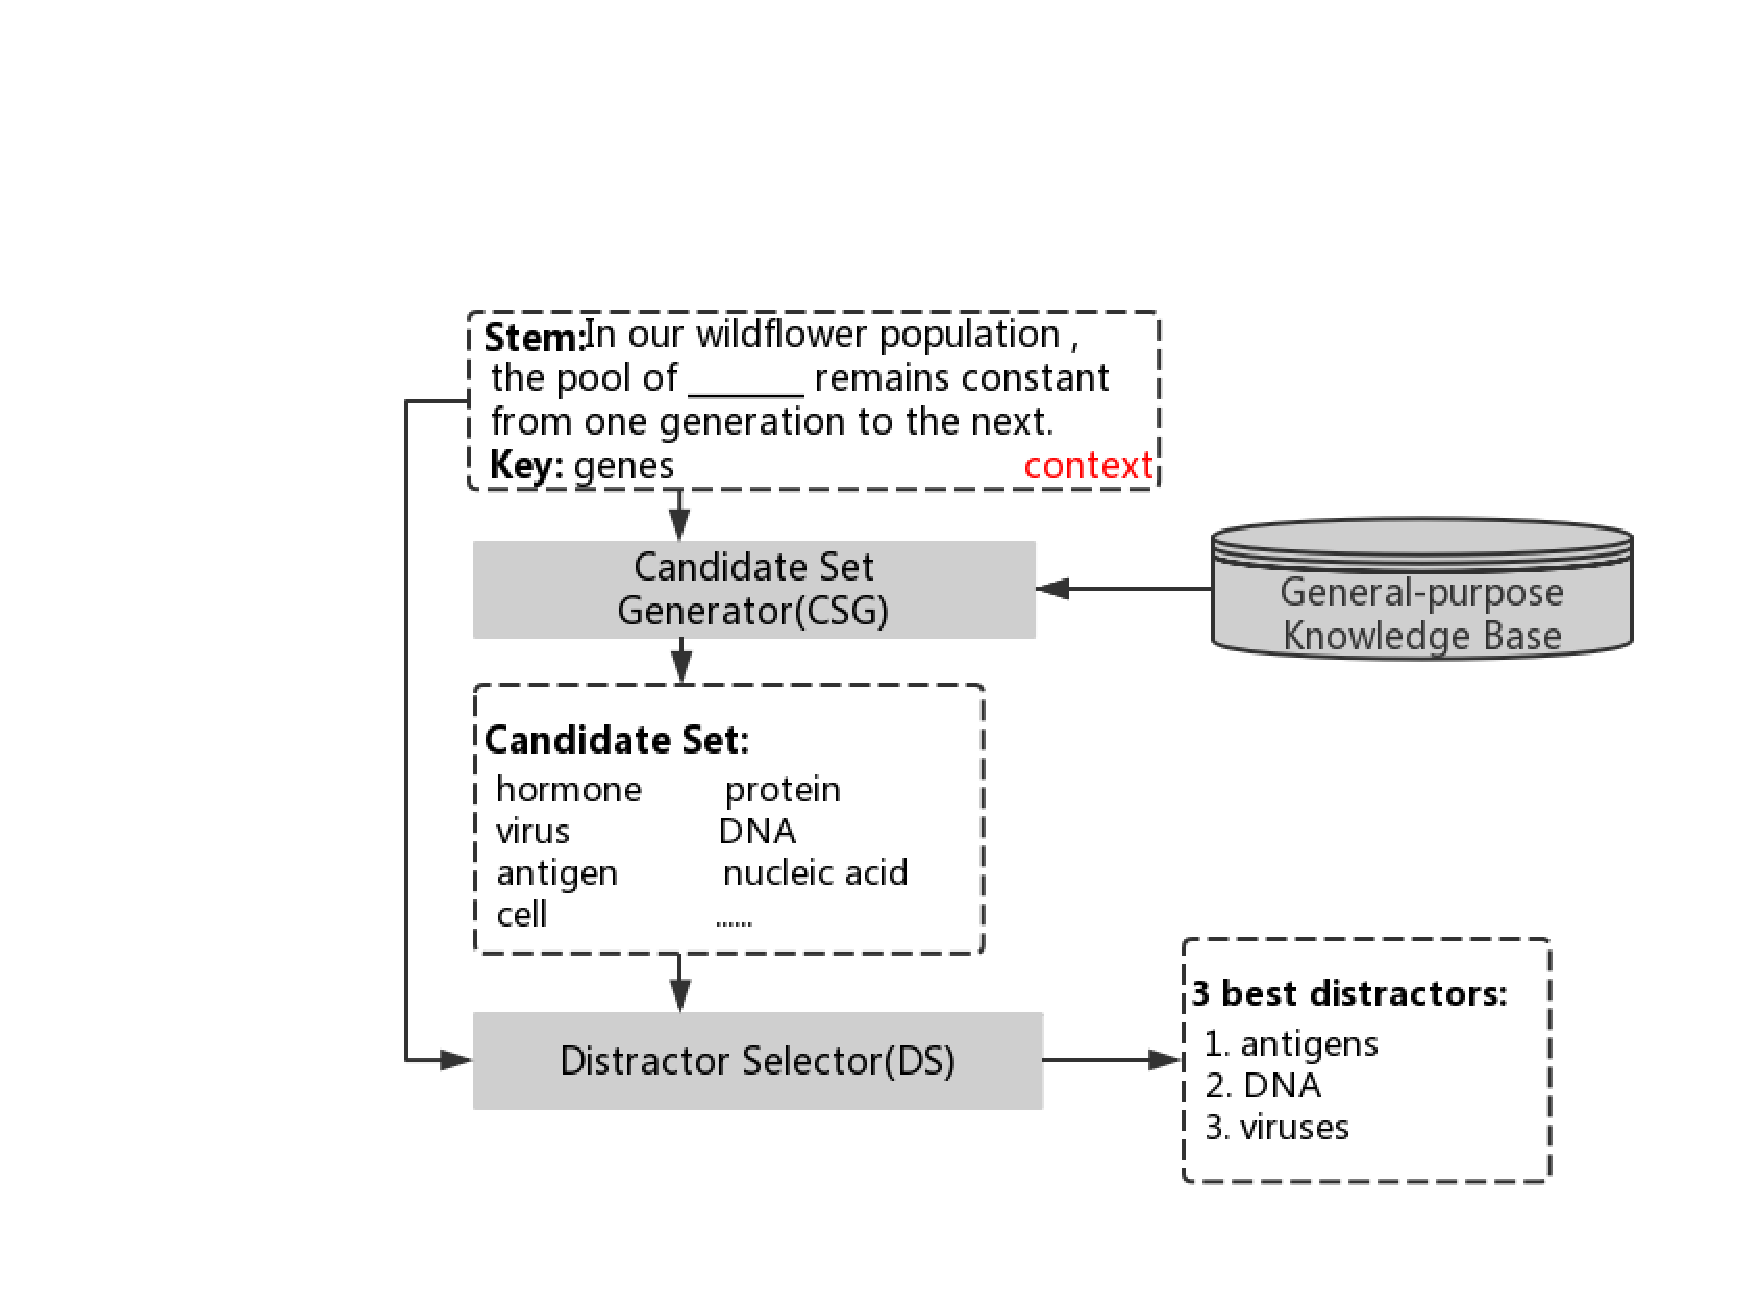
\includegraphics[width=1.0\columnwidth]{figure/csg_ds.eps}}
\caption{An overview of our framework.} \label{fig:framework}
\end{figure}
% \KZ{Maybe re-orient the pic to save some space?}

\subsection{Task Formulation}
Formally, given the stem $q$ and key $a$, the task of distractor generation is to generate $n$ most 
appropriate~(meet the requirement of plausibility and reliability) distractors $D = \{(d_i, s_i)\}$, $1\leq i\leq n$,
with predicted ranking scores $s_i$ in descending order.
%\KZ{I think you need to
%define what is ``approprite'' in a formal way.}
% We first retrieve $m$ candidates from a general-purpose knowledge base which are 
% defined as $A = \{(d_1, p_1), (d_2, p_2), \cdots,(d_m, p_m) \}$ where $d_i$ 
% is the $i$-th retrieved candidate and $p_i$ is the corresponding probability 
% obtained from knowledge base. Then our ranking model measures the score of 
% each candidate $d_i$ given stem $q$ and key $a$ and outputs a $n$-best 
% list $\{(d_1, s_1), (d_2, s_2), \cdots, (d_n, s_n)\}$ where $s_i$ represents 
% the ranking score.

\subsection{Candidate Set Generator (CSG)}
\label{sec:CSG}
%Knowledge base stores structured data, but it alone often lacks 
%context-sensitivity for this task. 
The proposed CSG explicitly leverages the observation that distractors to 
an open-domain cloze-style MCQ are often words or short phrases 
living in a knowledge base (e.g., Probase~\cite{wu2012probase}, WordNet~\cite{leacock1998combining}) and stored as \textit{nodes} in a way that they are connected with the key through a common \textit{parent node} (which we refer to as \textit{concept} later). Instead of enumerating all words in a huge 
domain-specific vocabulary in early approaches, such hierarchical structure in knowledge base allows us to extract candidate distractors by only considering a reasonably small number of concepts $C$ that are semantically related to the key, 
which can be efficiently identified using KB-specific interface.
% Stems cannot be used directly to facilitate the candidate retrieval process, 
% so the candidate set generator first extracts latent context $z$ from the stem $q$ and the key $a$.
% It further retrieves a candidate set $D$ from knowledge base efficiently based on $z$,
% and measures the probability distribution $P(d_i | z)$ over all retrieved candidates. 
% We use Probase due to its large coverage of real-world concepts, which is well-suited for DG in the open domain setting. 
% It contains more than millions of concept-instance relationships automatically extracted using syntactic patterns from billions of Web pages, more than any other existing knowledge bases(e.g. Freebase~\cite{Bollacker:2008:FCC:1376616.1376746}, WordNet~\cite{miller1998wordnet}).It also specifies the probability of each instance belonging to the concept, $P(w|c)$, as well as the probabilities of the reverse direction $P(c|w)$. Its hierarchical concept structure allows us to conduct context-dependent conceptualization (CDC)~\cite{kim2013context} on the key $a$ to handle potential polysemy, and find other entities belonging to the same concept-level in this hierarchical concept graph. 


Nevertheless, the specific meaning of the key varies given different stems. For example, given sentence: ``\textit{These survivors managed to swim to the \textbf{bank}},'' where \textit{\textbf{bank}} is the key, we would like to generate candidates like \textit{shore} rather than the more commonly used 
financial-related terms.
% We illustrate this process with a running example:
% \begin{itemize}
% 	\item Given a stem "In our wildflower population, the pool of \underline{\hbox to 8mm{}} remains constant from one generation to the next"
% \end{itemize}

% The topic distribution of the sentence formed by the stem and key 
% serves as the context information for conceptualizing each instance word. 
% With it, we estimate the concept distribution for the key by computing 
% the probability of each concept based on the topic distribution of the sentence. 
% The probability of concept $c$ given instance $w$ with its context by 
% considering the topic distribution topics is calculated as follows:
Inspired by the idea of context-dependent conceptualization~\cite{kim2013context}, we utilize a probabilistic topic model, LDA~\cite{Blei:2003:LDA:944919.944937}, to discover the latent topic distribution of the context as well as the topic distribution of all concepts in the concept set $C$. The posterior probability $p(c|a, q)$
of key $a$ belonging to concept $c$ conditioned on the stem $q$, is given by: 
\begin{align}
	p(c|a, q) &\propto p(c|a) \sum_{k=1}^K \pi_{a,q}^{(k)} ~ \gamma_{c}^{(k)}
	\label{eq:pc}
\end{align}
where $c$ is the concept, $\pi_{a,q}$ is the topic distribution of complete sentence formed by the stem and key, $\gamma_{c}$ denotes the topic distribution of concept $c$, $p(c|a)$ is the prior probability of $a$ belonging to $c$ corresponding to the specific choice of knowledge base, 
and $K$ is total number of topics. 
Intuitively, concepts whose topic distribution resembles that of the complete sentence will be weighted higher than others.
\begin{figure}[t]
\centering
\scalebox{1.0}{\includegraphics[width=1.0\columnwidth]{figure/probase.eps}}
\caption{A snippet of Probase. Instances are connected to concepts under \textit{is-A} relation.} \label{fig:probase}
\end{figure}
After obtaining the conditional probability $p(c|a, q)$ of all concepts in 
$C$, by following the descending chain of \textit{is-A} relation and 
collecting hyponyms of these concepts as in \figref{fig:probase}, we get a probability distribution over 
all entities subsumed by the concepts in $C$:
\begin{align}	
	p_{i} = p(d_i|a,q) \propto \sum_{c\in C} p(d_i|c) p(c|a,q)
	\label{eq:pd}
\end{align}
where the probability $p(d|c)$ is also known as 
typicality~\cite{wu2012probase}. 
The prior probability $p(c|a)$ and typicality $p(d|c)$ can be used
off-the-shelf in some KBs (e.g., Probase) while for some other KBs
(e.g., WordNet) it is not the case, which endows our framework with 
the flexibility to be combined with a broad class of KBs and 
to be customized with different ways of calculating these two probabilities.

Then we remove candidates that occur in the stem and finally the top $m$ candidates with largest probabilities form a candidate distractor set $D_0 = \{(d_1, p_1), (d_2, p_2), \cdots,(d_m, p_m) \}$. 

\subsection{Distractor Selector (DS)}
\label{sec:DS}
Given the previously constructed candidate distractor set $D_0$, the final $n$-best distractors are generated in the following steps.
\subsubsection{Feature Extractor}
\label{sec:FE}
Given a triplet ($q$; $a$; $d$) where $q$ is the stem, $a$ is the key and $d$ is a candidate distractor, 
our DS first transforms it into a feature vector $f(q,a,d)\in \mathbb{R}^l$, in which the features are defined below:
\begin{itemize}
%	\setlength{\itemsep}{1pt}
%\setlength{\parsep}{1pt}
%\setlength{\parskip}{1pt}
	% \item[-] \textit{Probase Score.} ~$p(d|a,z)$ from candidate set generator. 
	\item[-] \textit{Embedding Similarity:} ~Embedding similarity between $q$ and $d$ and the similarity between $a$ and $d$ calculated using Word2Vec, which is effective for finding semantically similar distractors~\cite{guo2016questimator}. We use the average word embedding as the sentence embedding. 
	\item[-] \textit{Contextual Embedding Similarity:} ~Cosine similarity between the ELMo~\cite{peters2018deep} embedding of $a$ and $d$. This feature is complementary to \textit{Emb Similarity} since Word2Vec only capture static blended semantic of words, of which the significance is verified in \secref{sec:res}.
	\item[-] \textit{Morphological Similarity:} ~Edit distance, token/character length difference, singular/plural consistency, absolute and relative length of $a$ and $d$'s longest common prefix/suffix/subsequence. These features measure the morphological similarity and are useful for cases such as abbreviation 
(e.g., DNA and RNA). 
	\item[-] \textit{POS Similarity:} ~Jaccard similarity between the 
POS tags of $a$ and that of $d$. The intuition is that good distractor 
should share similar linguistic property as the answer.
	\item[-] \textit{Frequency:} ~Average unigram frequency of $a$ and $d$. Frequency has been previously utilized as a proxy for word's difficulty level~\cite{article}. This feature aids model to select distractors with similar difficulty as $a$.
	\item[-] \textit{Compositional Similarity:} ~Jaccard similarity between token-level
unigram set and bigram set of $a$ and $d$. This feature is motivated 
by the observation that distractors might share tokens with answer.
	% \item[-] \textit{LM Score.} ~Conditional Probability of $d$ given $q$, $p(S) \approx \Pi_{i=1}^k p(w_i | w_1, \cdots, w_{i-1}, w_{i+1}, \cdots, w_k)$, predicted by language model. This is inspired by the previously proposed reliability checking approach of considering collocations involving the target word~\cite{jiang2017distractor, pino2008selection,smith2010gap}. 
	\item[-] \textit{Web-search Score:} ~Detail of this feature is described later in this section.
\end{itemize} 

% \textit{Embedding Similarity}, \textit{Contextual Embedding Similarity}, \textit{Morphological Similarity}, \textit{POS Similarity}, and \textit{Compositional Similarity} 
Features except \textit{Web-search Score} are integrated to mainly evaluate the plausibility of $d$ in various aspects and granularities. \textit{Web-search Score} is specifically introduced to assess
the validity of the sentence restored by each candidate in order to further strengthen reliability.  
% The Web includes all manners of textual data in vast quantities. 
% So we dare to assume that an \textit{(argument1, relation phrase, argument2)} 
% triple is more likely to be correct if it appears more frequently on the Web. 
% We also make the assumption that the validity of triple can be used to measure 
% the correctness of a sentence if the triple forms its main structure.
First, search results are retrieved from the web by passing the full sentence 
concatenated from $q$ and $d$ to the Bing search engine automatically. 
Then, we use ReVerb ~\cite{fader2011identifying} to 
extract \textit{(argument1, relation phrase, argument2)} triplets 
involving $d$ from the sentence formed by $q$ and 
$d$, $\{t_{11}, t_{12}, \cdots, t_{1n}\}$, 
as well as triplets in the titles and snippets returned by the search engine, 
$\{t_{21}, t_{22}, \cdots, t_{2m}\}$. 
After that, we calculate embedding similarities 
between triplets and keep the maximal score, 
$T(q,d)$, that represents the correctness of triplet extracted from a sentence:
% \KZ{Say more clearly how you compute hit(q,d).  Give a formula.}
\begin{equation*}
	T(q,d) = max_{\tiny \begin{array}{c}
	i\in \{1,2,\cdots,n\} \\ j \in \{1,2,\cdots,m\}
	\end{array}
	} EmbSim(t_{1i}, t_{2j}),
\end{equation*}
where $EmbSim(t_{1i}, t_{2j})$ represents the word2vec embedding similarity between $t_{1i}$ and $t_{2j}$.
If $T(q,d)$ is small, then the sentence restored with the distractor $d$ is unlikely, thus $d$ should be a reliable distracter. 

\subsubsection{Ranker}
\label{sec:AMMR}
Given the feature vector $f(q, a, d)\in \mathbb{R}^l$ where $q$ and 
$a$ are the stem and key of triplet $(q; a; D_g)$ in the dataset, 
we propose to utilize a feature-based learning-to-rank model, 
which is trained in a supervised manner and learns to assign higher
scores to those $d$'s within the ground-truth distractor set $D_g$ 
than those in $D_0-D_g$. Reasonable distractors outside of $D_g$ are 
likely to be close to ground-truth distractors in the feature space 
$\mathbb{R}^l$, which can implicitly guide the ranker to learn relative 
ranking of negative examples during training.

% We choose the list-wise ranker to be LambdaMART~\cite{burges2010from} in implementation due to its excellent performence in ranking task. The relevance score $rel_i(d)$ for candidate distractor $d$ with respective to a specific training triplet ($q_i$, $a_i$, $D_i$) is calculated based on average semantic distance between $d$ and ($a_i$, $D_i$):
% \begin{align}
% 	\label{eq:rel}
% 	&dist(d, w) = \frac{dist_{Emb}(d,w)+dist_{ELMo}(d,w)}{2} \\
% 	&rel_i(d) = 2^{1-avg(dist(d, a_i)+\sum_{j=1}^{|D_i|}dist(d, d_{ij}))} - 1
% \end{align}
% Where $d_{ij}$ is the $j$-th ground truth distractor in $D_i$, $dist(d,w)$ measures the averaged cosine distance of word2vec embedding and ELMo embedding between $d$ and $w$. Hence, distractors that has large discrepancy in semantic compared to answer and ground-truth distractors will be assigned a lower score. 
Note that we do not restrict the ranker to be any specific model. 
One can choose to implement it using any state-of-the-art point-wise, 
pair-wise or list-wise learning-to-rank models. Theoretically, 
training a learning-to-rank model requires a relevance score associated with 
each distractor, which is not available in existing cloze-style 
MCQ dataset. We remedy this by setting the relevance score for $d\in D_g$ as 1 
and for $d\in \{D_0-D_g\}$ as 0. For point-wise ranker, 
it reduces into a binary-classifier~\cite{liang2018distractor}. 
The major difference between point-wise ranking model and 
pair/list-wise ranking model is that the latter may learn latent 
feature patterns for discriminating between better or worse distractors 
through supervised training signal.

% We compute relevance score for negative examples that are not in $D_i$ using \eqnref{eq:rel} and set it to be $2^{2}-1=3$ for all $d_{ij}$ in $D_i$. 
% After obtaining the relevance score, the learning objective then amounts to maximizing the normalized discounted cumulative gain.~To make the training process more efficient and effective, following Liang~\shortcite{liang2018distractor}, we adopt a two-stage cascaded training strategy where the first stage ranker is a light-weight point-wise ranker trained with part of features in \secref{sec:FE} and the second
% stage ranker is a list-wise learning-to-rank model trained with all features. 

At test time, the ranking score $s_i$ for each candidate distractor $d_i$ 
predicted by the ranker is then used to sort the candidates in 
$D_0$ extracted by CSG and output the final $n$-best ranked list 
$D = \{(d_1, s_1), (d_2, s_2), \cdots, (d_n, s_n) \}$.
